% default values
\def\omegagh{10^2}  % omega_gh = omega_gu (Grenzfrequenz Hochpass bzw. untere Grenzfrequenz)
\def\omegagt{10^4}  % omega_gt = omega_go (Grenzfrequenz Tiefpass bzw. obere Grenzfreuquenz)

% Plot Umgebung:
\def\samples{41}

\def\xomegaordermin{0}
\def\xomegaordermax{6}
\def\xomegamin{1e\xomegaordermin}
\def\xomegamax{1e\xomegaordermax}

\def\yPhimin{-90} % 0.8 für Platz für Steigungsdreiecke
\def\yPhimax{+90} % 2^0.5 für Platz

% Bandpass (Tiefpass 1. Ord + Hochpass 1. Ord) - Phasengang
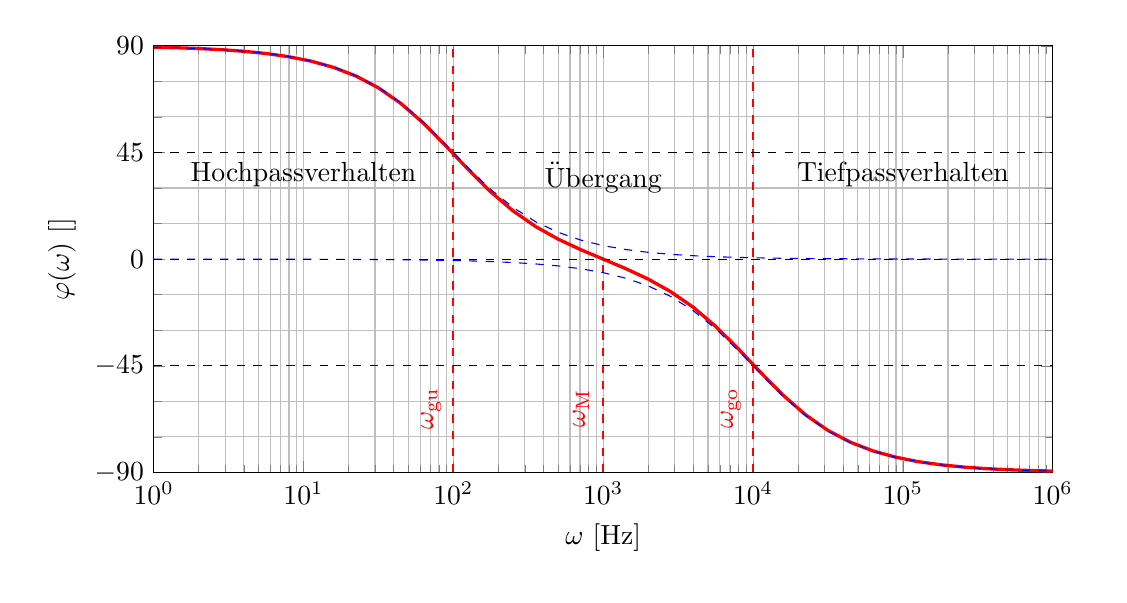
\begin{tikzpicture}[x=1mm,y=1mm] % gilt für tikz-coordinaten außerhalb der axis-environment
    \draw[draw=none] (-16,-13) rectangle (120,36); % Bildrahmen, Koordinatenbezug auf (0,0) des \begin{axis}...\end{axis} pgfplots, für
    \begin{semilogxaxis}[
        %title={Bandpass},
        xlabel={$\omega\ [\mathrm{Hz}]$},
        ylabel={$\varphi(\omega)\ [\degree]$},
        xmin=\xomegamin, xmax=\xomegamax,
        ymin=\yPhimin, 
        ymax=\yPhimax,   % \ymin needed as macro to draw ycomb with node-text from x-axis to plot intersection
        domain=\xomegamin:\xomegamax,
        samples=\samples,
        grid=minor,
        width=13cm,
        height=7cm,
        minor y tick num= 2,
        ytick distance=45,
    ]
        % Plot: Phi(omega) = Phi_h(omega) + Phi_t(omega)
        \addplot+[mark=none,very thick,red,]     {atan(\omegagh/x) + atan(-x/\omegagt)}; % Phi(omega) = arctan(omegagh/x) + arctan(-x/omegagt)

        % Grenzfrequenzen, Mittenfrequenz
        \addplot+[dashed,mark=none,thick,red,] coordinates {(\omegagh,\yPhimin)(\omegagh,\yPhimax)}  node [pos=0.15,sloped,style={yshift=8pt}] {$\omega_{\mathrm{gu}}$}; % Grenzfrequenz
        \addplot+[dashed,mark=none,thick,red,] coordinates {(\omegagt,\yPhimin)(\omegagt,\yPhimax)}  node [pos=0.15,sloped,style={yshift=8pt}] {$\omega_{\mathrm{go}}$}; % Grenzfrequenz             
        \addplot+[dashed,mark=none,thick,red,] coordinates {((\omegagh*\omegagt)^0.5,\yPhimin)((\omegagh*\omegagt)^0.5,0)}  node [pos=0.3,sloped,style={yshift=8pt}] {$\omega_{\mathrm{M}}$}; % Mittenfrequenz

        \addplot+[mark=none,thin,blue,dashed]     {atan(\omegagh/x)}; % ideal Hochpass
        \addplot+[mark=none,thin,blue,dashed]     {atan(-x/\omegagt)}; % ideal Tiefpass

        % Nicht automatisch, trotz ytick distance = 45, minor y tick num=2, grid=minor
        \addplot+[dashed,mark=none,black,]  coordinates { (\xomegamin, 0) (\xomegamax, 0) };%  node [pos=0.1,sloped,yshift=8pt] {$0\ \degree$};
        \addplot+[dashed,mark=none,black,]  coordinates { (\xomegamin, 45) (\xomegamax, 45) };%  node [pos=0.1,sloped,yshift=8pt] {$+45\ \degree$};
        \addplot+[dashed,mark=none,black,]  coordinates { (\xomegamin, -45) (\xomegamax, -45) };%  node [pos=0.1,sloped,yshift=8pt] {$-45\ \degree$};            

        % Bereiche
        \node at (10^1,45) [anchor=north] {Hochpassverhalten};
        \node at (10^3,45) [anchor=north] {Übergang};
        \node at (10^5,45) [anchor=north] {Tiefpassverhalten};

    \end{semilogxaxis}
\end{tikzpicture}